% SSW 590 Group 1 DevOps IT Manual (living manual, one chapter per module).
% Built from the course Canvas template (2026F-SSW-590-DevOps-canvas-template.zip,
% template version 1.3, by Darian Muresan). One chapter per file; see devopsAIAgentGuide.tex.
\documentclass[12pt]{cornell}

\usepackage[T1]{fontenc}
\usepackage{lmodern}
\usepackage{xspace}
\usepackage{xcolor}
\usepackage{graphicx}
\usepackage{fancyhdr}
\usepackage{amsmath,amssymb}
\usepackage{array}
\usepackage{booktabs}
\usepackage{longtable}
\usepackage{tabularx}
\usepackage{ltablex}
\keepXColumns
\usepackage{enumitem}
\usepackage{listings}
\usepackage{minted}
\usepackage{tcolorbox}
\usepackage{makeidx}
\usepackage{tikz}
\usetikzlibrary{shapes.multipart,arrows.meta,positioning}
\usepackage[colorlinks=true,citecolor=blue,linkcolor=blue,urlcolor=blue]{hyperref}
\usepackage[acronym,toc]{glossaries}

\makeindex
\makeglossaries
\newacronym{ai}{AI}{artificial intelligence}
\newacronym{ci}{CI}{continuous integration}
\newacronym{cd}{CD}{continuous delivery or continuous deployment}
\newacronym{iac}{IaC}{infrastructure as code}
\newacronym{slo}{SLO}{service-level objective}
\newglossaryentry{automation}{name={automation},description={A repeatable, version-controlled procedure executed by software rather than undocumented manual steps}}
\newglossaryentry{container}{name={container},description={An isolated, runnable instance of a container image that packages an application with its dependencies}}
\newglossaryentry{containerimage}{name={container image},description={An immutable, layered template built from a Dockerfile from which containers are started}}
\newglossaryentry{deployment}{name={deployment},description={The controlled delivery of a versioned change to an environment}}
\newglossaryentry{evidence}{name={evidence},description={A retained record of an actual execution, observation, or review}}
\newglossaryentry{kanban}{name={Kanban board},description={A visual workflow board with columns such as To Do, In Progress, and Complete, used to make work and work-in-progress visible}}
\newglossaryentry{observability}{name={observability},description={The ability to infer system behavior from signals such as logs, metrics, traces, and health checks}}
\newglossaryentry{pipeline}{name={pipeline},description={An automated sequence that builds, tests, packages, and/or deploys a change}}
\newglossaryentry{rollback}{name={rollback},description={A controlled return to a known acceptable version or state after a failed or harmful change}}
\newglossaryentry{runbook}{name={runbook},description={A documented operational procedure for a repeatable task or incident response}}
\newglossaryentry{synonyms}{name={synonyms},description={Equivalent terms used in this assignment; record preferred terms to avoid ambiguity in instructions and evidence}}
\newacronym{aws}{AWS}{Amazon Web Services}
\newacronym{ec2}{EC2}{Amazon Elastic Compute Cloud}
\newacronym{ami}{AMI}{Amazon Machine Image}
\newacronym{uml}{UML}{Unified Modeling Language}
\newacronym{dora}{DORA}{DevOps Research and Assessment}
\newacronym{swot}{SWOT}{strengths, weaknesses, opportunities, and threats}
\newglossaryentry{securitygroup}{name={security group},description={A stateful virtual firewall attached to an AWS instance that lists the inbound and outbound traffic it allows}}
\newglossaryentry{userdata}{name={user data},description={A script supplied when an EC2 instance is launched that runs once as root at first boot}}
\newglossaryentry{texlive}{name={TeX Live},description={A cross-platform distribution of TeX, LaTeX, and their packages; Overleaf compiles projects with it}}
\newacronym{tls}{TLS}{Transport Layer Security}
\newacronym{dns}{DNS}{Domain Name System}
\newglossaryentry{gitea}{name={Gitea},description={A self-hosted Git service with issues, pull requests, and organizations}}
\newglossaryentry{compose}{name={Docker Compose},description={A tool that runs a multi-container application from a versioned YAML file}}
\newglossaryentry{persistence}{name={persistence},description={Data surviving replacement of the container that uses it, because it lives on a mounted volume}}


\definecolor{devopsBlue}{RGB}{31,78,121}
\definecolor{devopsGreen}{RGB}{46,125,50}
\definecolor{devopsRed}{RGB}{183,28,28}
\definecolor{devopsGray}{RGB}{90,90,90}
\definecolor{devopsLightBlue}{RGB}{232,240,247}

\newcommand{\AssignmentTitle}{Group 1 DevOps IT Manual}
\newcommand{\AssignmentNumber}{4}
\newcommand{\DocumentVersion}{0.1}
\newcommand{\DocumentStatus}{Draft: Gitea Chapter in Progress}
\newcommand{\CourseNumber}{SSW 590}
\newcommand{\CourseName}{DevOps}
\newcommand{\Instructor}{David Darian Muresan, Ph.D.}
\newcommand{\StudentName}{Group 1: Brahmi Dalvi and Sakshi Deshpande}
\newcommand{\Organization}{Stevens Institute of Technology}
\newcommand{\DocumentDate}{October 12, 2026}
\newcommand{\DueDate}{set by the LMS}
\newcommand{\VERSION}{Version \DocumentVersion}
\newcommand{\RepoURL}{https://github.com/brahmi9811/ssw-590-group1}
% Placeholders: set once the domain is claimed and the Gitea org/repo exist.
\newcommand{\GiteaHost}{git.ssw590-g1.tech}
\newcommand{\GiteaURL}{https://\GiteaHost}
\newcommand{\GiteaRepoURL}{\GiteaURL/startup/product}

\hypersetup{
  pdftitle={\CourseNumber\ --- \AssignmentTitle},
  pdfauthor={\StudentName},
  pdfcreator={Group 1, with Anthropic Claude Code},
  pdfsubject={Group 1 DevOps IT manual (Gitea)},
  pdfkeywords={DevOps, Gitea, HTTPS, firewall, evidence}
}

\newcolumntype{Y}{>{\raggedright\arraybackslash}X}
\newcolumntype{L}[1]{>{\raggedright\arraybackslash}p{#1}}
\setlength{\tabcolsep}{4pt}
\renewcommand{\arraystretch}{1.12}
\setlength{\LTpre}{6pt}
\setlength{\LTpost}{6pt}

% Stable IDs make activity, evidence, and artifact references durable.
\newcommand{\ArtifactLabel}[2]{\phantomsection\label{#1:#2}}
\newcommand{\ArtifactID}[2]{\texttt{#2}\ArtifactLabel{#1}{#2}\index{#1!#2}}
\newcommand{\ArtifactRef}[2]{\hyperref[#1:#2]{\texttt{#2}}}
\newcommand{\EvidenceID}[1]{\ArtifactID{Evidence}{#1}}
\newcommand{\EvidenceRef}[1]{\ArtifactRef{Evidence}{#1}}
\newcommand{\ChapterLabel}[1]{\label{Chapter:#1}}
\newcommand{\ChapterRef}[1]{\hyperref[Chapter:#1]{Chapter~\ref*{Chapter:#1}}}
\newcommand{\StatusPass}{\textbf{\footnotesize\textcolor{devopsGreen}{PASS}}}
\newcommand{\StatusPending}{\textbf{\footnotesize\textcolor{devopsGray}{PENDING}}}
\newcommand{\StatusFail}{\textbf{\footnotesize\textcolor{devopsRed}{FAIL}}}
% Marks text a team member still has to supply. Never leave one in a submitted PDF.
\newcommand{\Todo}[1]{\textcolor{devopsRed}{\textbf{[TODO: #1]}}}

\newtcolorbox{devopsNote}[1][]{
  colback=devopsLightBlue, colframe=devopsBlue, boxrule=0.6pt, arc=1mm, title={#1}
}

\lstset{
  backgroundcolor=\color{white}, basicstyle=\ttfamily\footnotesize,
  breaklines=true, frame=single, keywordstyle=\color{blue},
  commentstyle=\color{devopsGreen}, numbers=left, numbersep=6pt,
  numberstyle=\tiny\color{devopsGray}, showstringspaces=false,
  stringstyle=\color{devopsRed}, tabsize=2
}
\setminted{fontsize=\footnotesize, breaklines, breakanywhere, frame=lines, framesep=2mm}

\setlength{\emergencystretch}{3em}
\changenormalspacing{\singlespacing}
\begin{document}
\pagenumbering{roman}
\singlespacing
\title{\CourseNumber\ --- \CourseName\\[0.5em]\large \AssignmentTitle\\[1.5em]\normalsize\VERSION\\\DocumentStatus}
\author{\StudentName\\\Organization}
\conferraldate{}{\DocumentDate}
\copyrightholder{\Organization}
\copyrightyear{2026}
\maketitle
\makecopyright

\cleardoublepage
\phantomsection
\chapter*{Template Attribution}
\ChapterLabel{TemplateAttribution}
\addcontentsline{toc}{chapter}{Template Attribution}
\markboth{Template Attribution}{Template Attribution}
\index{template attribution}
\index{Muresan, Darian}
This manual is built from the SSW~590 DevOps assignment template (version
1.3, distributed through Canvas), developed by \textbf{Darian Muresan, Ph.D.},
in conjunction with \textbf{OpenAI Codex} and \textbf{Anthropic Claude Code}.

\clearpage
\begin{abstract}This is Group~1's living DevOps IT manual for SSW~590. It records what the
group actually built, tested, and learned, one chapter per course module. The
first chapter documents the startup's Gitea work hub: a student-pack domain,
a version-pinned Gitea deployment, HTTPS with automated certificate renewal, a
minimal firewall exposure, and an issue-to-reviewed-merge team workflow. Results
are stated only where they were observed. The one thing not observed, the first
automatic renewal of the production certificate (expected between December 13 and
15, 2026, after the due date), is labeled as such.
\end{abstract}
\chapter*{Document History}
\addcontentsline{toc}{chapter}{Document History}
\index{document history}
\section*{How to Use This Chapter}
Add the newest approved change at the top. Retain every approved entry and
link each entry to the changed chapter, table, figure, or controlled artifact.
Every entry must say whether the Hosts and Passwords tables changed.
Author initials: BD = Brahmi Dalvi, SD = Sakshi Deshpande, CC = Claude Code
(AI assistant; see the AI Prompt Log).

\begin{tabularx}{\linewidth}{L{3.1cm}L{2.2cm}YL{2.0cm}}
\caption{Document Update History\label{Table:DocumentHistory}}\\
\toprule \textbf{Date / Version} & \textbf{Author Initials} & \textbf{Change} & \textbf{Changed At}\\ \midrule
\endfirsthead
\multicolumn{4}{l}{\small\itshape Document Update History (continued)}\\
\toprule \textbf{Date / Version} & \textbf{Author Initials} & \textbf{Change} & \textbf{Changed At}\\ \midrule
\endhead \bottomrule \endlastfoot
October 12, 2026 / 0.1 & BD, CC & Initial setup: created the separate IT manual from the course Canvas template (version 1.3, one chapter per file, template guides retained as appendices), the Gitea chapter outline with the eight rubric-aligned subsections and an extra-credit subsection, and the Hosts and Passwords tables. Hosts and Passwords tables created, with no real hosts or secrets recorded yet. No infrastructure exists yet; every evidence item is pending. & \ChapterRef{Introduction}, \ChapterRef{HostsPasswords}, \ChapterRef{Gitea}\\
\end{tabularx}

\contentspage
\tablelistpage
\figurelistpage


\setcounter{page}{1}
\pagenumbering{arabic}
\pagestyle{fancy}
\fancyhf{}
\renewcommand{\chaptermark}[1]{\markboth{#1}{}}
\lhead{\small IT Manual}
\chead{\small\nouppercase{\leftmark}}
\rhead{\small\thepage}
\lfoot{\small\CourseNumber}
\cfoot{\small\copyright\ \Organization}
\rfoot{\small\VERSION}
\renewcommand{\headrulewidth}{0.4pt}
\renewcommand{\footrulewidth}{0.4pt}

\chapter{Introduction}
\ChapterLabel{Introduction}
\index{introduction}
\index{IT manual}

\section{Purpose}
This is Group~1's operational IT manual for the SSW~590 startup. It is a living
record: one chapter is added per delivered capability, and the compiled PDF is
the only artifact submitted for each assignment. It is separate from the
earlier assignment report in the \texttt{report/} folder of the repository.

\section{Team and Repository}
\begin{tabularx}{\linewidth}{L{3.6cm}Y}
\toprule \textbf{Item} & \textbf{Value}\\ \midrule
Group & Group 1\\
Members & Brahmi Dalvi (BD), Sakshi Deshpande (SD)\\
Course repository & \url{\RepoURL}\\
Team Gitea & \href{\GiteaURL}{\texttt{\GiteaURL}}; organization \href{\GiteaURL/group1-startup}{\texttt{group1-startup}}, product repository \href{\GiteaRepoURL}{\texttt{twintrack}}\\ \bottomrule
\end{tabularx}

\section{Chapter Map}
\begin{tabularx}{\linewidth}{L{3.6cm}Y}
\toprule \textbf{Where} & \textbf{Content}\\ \midrule
\ChapterRef{HostsPasswords} & Hosts and Passwords tables (hints only)\\
\ChapterRef{Gitea} & Startup foundation with Gitea (course Chapter~2)\\ \bottomrule
\end{tabularx}

\section{Repository Layout}
\begin{minted}{text}
assignment-4/manual/   this LaTeX manual (source stays in the team; submit only the PDF)
assignment-4/gitea/    versioned, non-secret deployment files (compose, proxy config)
assignment-4/*.md      work split and per-person instructions
report/                earlier submitted assignment (do not modify)
\end{minted}

\chapter{Hosts and Passwords}
\ChapterLabel{HostsPasswords}
\index{hosts table}
\index{passwords table}
Keep both tables current; a missing or stale table costs 10 points. The
Passwords table holds \emph{hints and vault references only}: never a
password, derivation key, recovery code, token, or private key.

\section{Hosts}
\begin{tabularx}{\linewidth}{L{2.6cm}L{1.8cm}L{1.6cm}L{2.2cm}L{1.6cm}Y}
\caption{Hosts\label{Table:Hosts}}\\
\toprule \textbf{Hostname} & \textbf{Role} & \textbf{Provider} & \textbf{Address / DNS} & \textbf{Exposed ports} & \textbf{Owner / HTTPS URL / backup}\\ \midrule
\endfirsthead
\toprule \textbf{Hostname} & \textbf{Role} & \textbf{Provider} & \textbf{Address / DNS} & \textbf{Exposed ports} & \textbf{Owner / HTTPS URL / backup}\\ \midrule
\endhead \bottomrule \endlastfoot
\Todo{git host} & Gitea + TLS proxy & \Todo{AWS or DO} & \Todo{IP, DNS} & \Todo{443, 80?, admin SSH} & \Todo{owner; \GiteaURL; none yet}\\
\end{tabularx}

\section{Passwords (hints only)}
\begin{tabularx}{\linewidth}{L{3cm}L{2cm}Y L{2.4cm}}
\caption{Passwords (hints only)\label{Table:Passwords}}\\
\toprule \textbf{Service / account} & \textbf{Owner} & \textbf{Vault reference or hint (no secret)} & \textbf{Privilege / MFA}\\ \midrule
\endfirsthead
\toprule \textbf{Service / account} & \textbf{Owner} & \textbf{Vault reference or hint (no secret)} & \textbf{Privilege / MFA}\\ \midrule
\endhead \bottomrule \endlastfoot
\Todo{Gitea admin} & \Todo{} & \Todo{where the real credential lives} & \Todo{admin / MFA?}\\
\end{tabularx}

\chapter{Startup Foundation with Gitea}
\ChapterLabel{Gitea}
\index{Gitea}
\index{startup DevSecOps process}

\section{Overview and Status}
This chapter answers the course manual's Chapter~2 \cite{DosManual}: the
startup's Gitea work hub with a student domain, HTTPS, minimal public
exposure, and persistent data. The eight numbered subsections below match the
eight rubric rows (100 points) in the same order. Optional backup and restore
evidence is a separate extra-credit subsection and is not part of the eight; it is optional and has no owner; the group will decide later whether time allows it.

\begin{devopsNote}[Provider status]
The assignment specifies a DigitalOcean Droplet. Group~1 asked the instructor
whether AWS could be used instead. On October 12, 2026 (8:36\,pm, Canvas
message ``Gitea Assignment --- Question on Cloud Provider (Group 1)'') the
instructor replied that any hosting service is allowed, including AWS or the
group's own servers, \textbf{as long as they are available online and can be
used by the TA and the instructor to test the assignments.} Group~1 therefore
uses AWS. The deployment must stay reachable and testable by the TA and
instructor until grading is complete.
\end{devopsNote}

\begin{tabularx}{\linewidth}{L{5.2cm}L{1.4cm}L{1.6cm}Y}
\caption{Rubric rows, owners, and status\label{Table:GiteaStatus}}\\
\toprule \textbf{Subsection} & \textbf{Points} & \textbf{Owner} & \textbf{Status}\\ \midrule
\endfirsthead
\toprule \textbf{Subsection} & \textbf{Points} & \textbf{Owner} & \textbf{Status}\\ \midrule
\endhead \bottomrule \endlastfoot
Student Pack domain and DNS & 10 & BD & \StatusPending\\
Pinned Gitea deployment & 10 & BD & \StatusPending\\
Database and persistence & 10 & SD & \StatusPending\\
HTTPS and certificate renewal & 15 & BD & \StatusPending\\
Firewall and external exposure & 15 & BD & \StatusPending\\
Startup team workflow & 20 & SD & \StatusPending\\
Architecture and operation & 5 & SD & \StatusPending\\
Manual quality and controls & 15 & SD & \StatusPending\\
Extra credit: backup and restore (optional) & up to 20 & unassigned & \StatusPending\\
\end{tabularx}

\section{Required Subsections}
% ======================================================================
% Region: giteaDomainDns (single owner; edit only your own region)
\subsection{Student Pack domain and DNS (10 points)}
\label{Section:giteaDomainDns}
\index{Gitea!student pack domain and dns}
\textbf{Owner:} BD. Domain registration: \StatusPass{} (order confirmed, \$0.00). Stored card removed: \StatusPass{}. DNS record and public-resolver lookup: \StatusPass{}. Teammate lookup and HTTPS link: \StatusPending{}.

\paragraph{Offer and eligibility.}
The domain comes from the GitHub Student Developer Pack, which lists domain
offers from Namecheap, Name.com, and .TECH Domains \cite{GitHubPackDomains}.
The group's Student Pack is approved on Brahmi Dalvi's GitHub account. The
Namecheap offer was started first but its GitHub authorization page requested
the \texttt{repo} scope (read and write access to all public and private
repositories), which the group judged too broad for a domain claim, so it was
cancelled. The Name.com Education Pack authorization requested ``public data
only'' and was accepted.

\paragraph{Domain and costs.}
\begin{tabularx}{\linewidth}{L{4.2cm}Y}
\caption{Domain registration facts\label{Table:DomainFacts}}\\
\toprule \textbf{Item} & \textbf{Value}\\ \midrule
\endfirsthead
\toprule \textbf{Item} & \textbf{Value}\\ \midrule
\endhead \bottomrule \endlastfoot
Domain & \texttt{ssw590-g1.tech}, registered at Name.com, order \#28974415. The confirmation email arrived Thursday, October 15, 2026 at 00:36 (mailbox local time) and gives the order date as October 14, 2026; the one-day difference is consistent with Name.com stamping the date in a different time zone, which we did not confirm\\
Planned Gitea hostname & \texttt{\GiteaHost} (A record created, see below)\\
First-year cost & \$0.00 (cart total \$0.00; the regular price shown struck through in the cart was \$89.99)\\
Renewal cost & \$89.99 (``Renew for \$89.99'' on the domain page)\\
Expiration & October 15, 2027\\
Automatic renewal & OFF (turned off after registration)\\
Extras declined & Domain Safe Pro (\$7.99/year); the free Domain Safe plan (domain lock, WHOIS privacy, free SSL certificate) is included\\
\end{tabularx}
The order summary after checkout also shows a struck-through \$7.99 next to the
domain; the group did not investigate that figure and relies on the \$0.00
total and the \$89.99 renewal price shown on the domain page.
Figure~\ref{Fig:DomainOrder} shows the completed order and
Figure~\ref{Fig:DomainDetails} shows the domain page after automatic renewal
was turned off.

\begin{figure}[htbp]
\centering
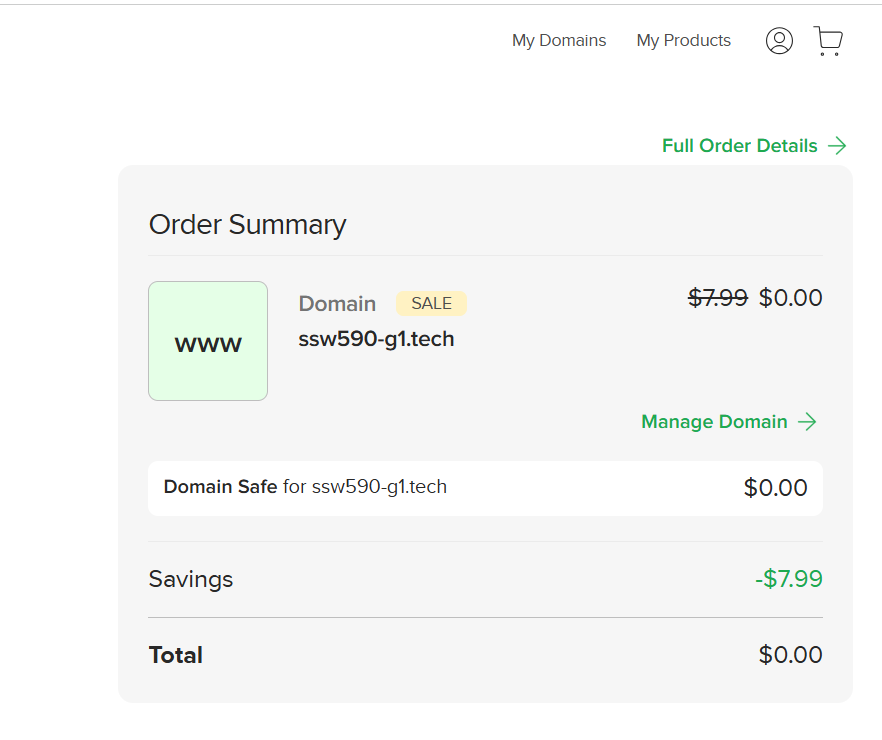
\includegraphics[width=0.7\linewidth]{../evidence/02-namecom-order-summary-ssw590-g1-tech-total-0.00-2026-10-15.png}
\caption{Name.com order summary, October 15, 2026: domain and free Domain Safe, total \$0.00.}
\label{Fig:DomainOrder}
\end{figure}

\begin{figure}[htbp]
\centering
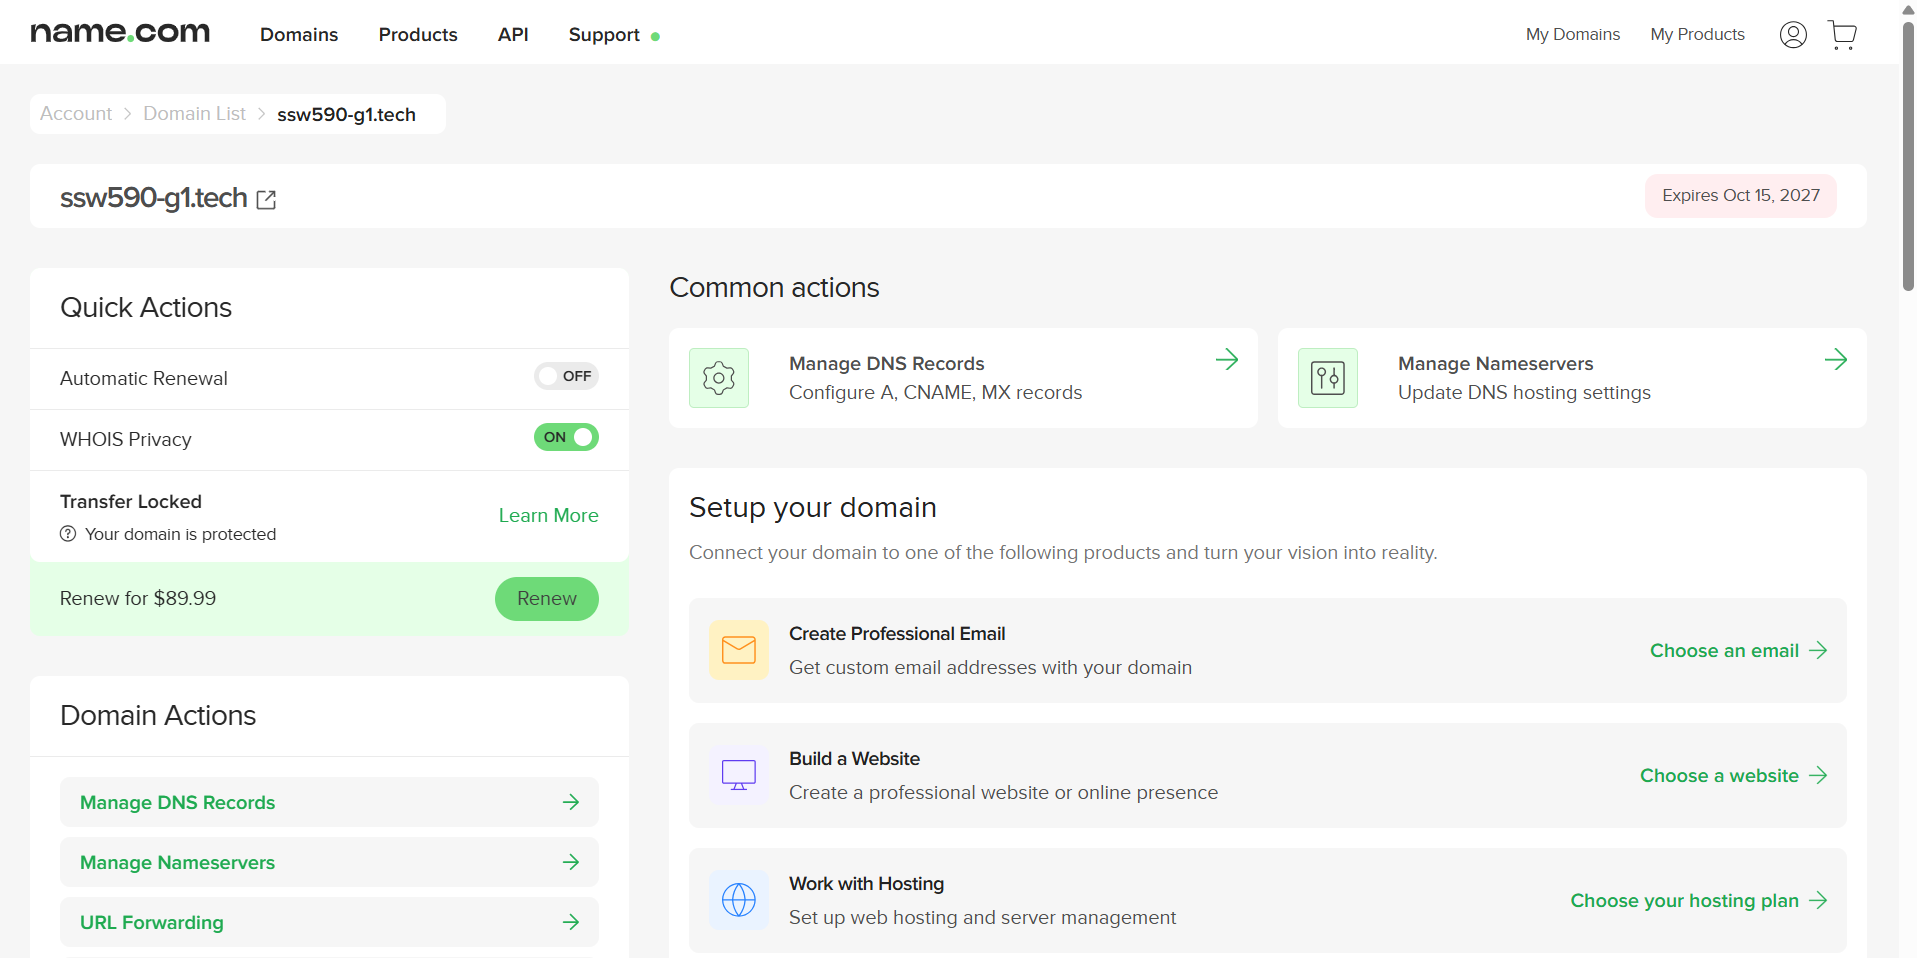
\includegraphics[width=\linewidth]{../evidence/04-namecom-domain-details-expires-2027-10-15-autorenew-OFF-2026-10-15.png}
\caption{Domain page, October 15, 2026: expires October 15, 2027, automatic renewal OFF, renewal price \$89.99.}
\label{Fig:DomainDetails}
\end{figure}

\paragraph{Renewal tracking.}
The group does not plan to renew: the domain is needed only through grading,
and the TA and instructor must be able to reach the service until then. Expiry
is October 15, 2027. \Todo{name the owner and calendar reminder for this date}

\paragraph{DNS record.}
In Name.com's DNS manager the group created one record, \texttt{A git.ssw590-g1.tech
52.73.254.36} with TTL 300 (Figure~\ref{Fig:DnsRecord}). The address is the Elastic
IP of the EC2 instance described in the deployment subsection. No AAAA record was
created, because the deployment is IPv4 only. The domain uses Name.com's own
nameservers (\texttt{ns1bqx}, \texttt{ns2kry}, \texttt{ns3jmt}, \texttt{ns4ksy}
\texttt{.name.com}).

\begin{figure}[htbp]
\centering
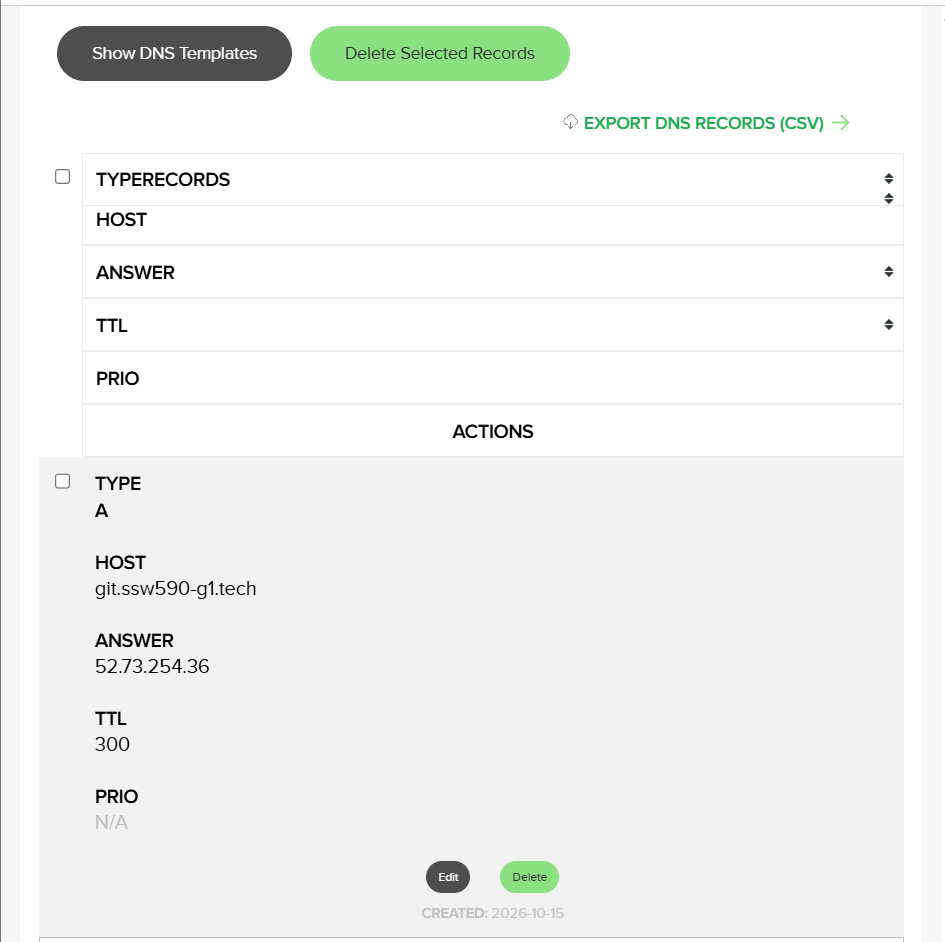
\includegraphics[width=0.6\linewidth]{../evidence/10-namecom-dns-a-record-git-ssw590-g1-tech-2026-10-15.png}
\caption{Name.com DNS records for \texttt{ssw590-g1.tech}, October 15, 2026: one A record for \texttt{git}.}
\label{Fig:DnsRecord}
\end{figure}

\paragraph{Lookup result.}
At 17:30:34 UTC on October 15, 2026 the name resolved to the expected address
through three public resolvers (expected: \texttt{52.73.254.36}; actual: the same).
\begin{center}
\begin{tabular}{lll}
\toprule \textbf{Resolver} & \textbf{Result for \texttt{\GiteaHost}} & \textbf{TTL}\\ \midrule
8.8.8.8 (Google) & A 52.73.254.36 & 300\\
1.1.1.1 (Cloudflare) & A 52.73.254.36 & 300\\
9.9.9.9 (Quad9) & A 52.73.254.36 & 300\\ \bottomrule
\end{tabular}
\end{center}
These lookups were run from Brahmi Dalvi's computer through public resolvers; they
were not run by a teammate on a separate network, so the independent-lookup
wording of the assignment is met only in that sense.
\Todo{optional: a teammate repeats the lookup (for example \texttt{nslookup \GiteaHost{} 8.8.8.8}) from another network and the result is added}.
The HTTPS hostname link will resolve once Gitea and the proxy are deployed.
\Todo{add the clickable HTTPS link once the site is live}

\paragraph{Payment safeguards.}
Name.com required a card even for the \$0.00 order. To avoid an unintended
renewal charge, the group turned automatic renewal off and deleted the stored
payment profile; the billing page then reads ``No saved payment profiles''
(evidence file \texttt{05-namecom-billing-no-saved-payment-profiles-2026-10-15.png}).
The confirmation email shows order \#28974415 with an order total of \$0.00
(evidence file \texttt{06-namecom-order-confirmed-email-order-28974415-received-2026-10-15-0036.png}). \Todo{after a few days, check the card statement and record whether any charge appeared}

% ======================================================================
% Region: giteaDeployment (single owner; edit only your own region)
\subsection{Pinned Gitea deployment (10 points)}
\label{Section:giteaDeployment}
\index{Gitea!pinned gitea deployment}
\textbf{Owner:} BD. \StatusPending{} No evidence recorded yet.

\textbf{Required content (from the course manual):}
\begin{itemize}[nosep]
  \item Droplet/EC2 and Gitea image versions, image source (Docker Hub \texttt{gitea/gitea})
  \item Deployment commands, restart policy, persistent mounts, proxy connection
  \item Redacted Compose excerpt and link to \texttt{gitea/docker-compose.yml} in the team repository
  \item Steps another team could repeat
\end{itemize}

\Todo{write the explanation, then add dated, labeled, sanitized evidence (expected vs.\ actual). A screenshot alone does not replace an explanation. Never claim a test that was not run.}

% ======================================================================
% Region: giteaDatabase (single owner; edit only your own region)
\subsection{Database and persistence (10 points)}
\label{Section:giteaDatabase}
\index{Gitea!database and persistence}
\textbf{Owner:} SD. \StatusPending{} No evidence recorded yet.

\textbf{Required content (from the course manual):}
\begin{itemize}[nosep]
  \item \textbf{Decision (final, team, October 12, 2026): SQLite.} Record the settings, the database-file path under the persistent \texttt{/data} volume, the volume mount, and why no database secret exists. Justify: two-person team, no extra container or credential, simple consistent backup; note it may not suit higher concurrency
  \item Repository and issue identifiers created before the test
  \item Exact container-replacement command (volumes kept), before/after evidence, conclusion
  \item Not applicable: PostgreSQL is not used, so there is no database port, healthcheck, or database secret to document
\end{itemize}

\Todo{write the explanation, then add dated, labeled, sanitized evidence (expected vs.\ actual). A screenshot alone does not replace an explanation. Never claim a test that was not run.}

% ======================================================================
% Region: giteaHttps (single owner; edit only your own region)
\subsection{HTTPS and certificate renewal (15 points)}
\label{Section:giteaHttps}
\index{Gitea!https and certificate renewal}
\textbf{Owner:} BD. \StatusPending{} No evidence recorded yet.

\textbf{Required content (from the course manual):}
\begin{itemize}[nosep]
  \item Comparison of two certificate options and the justification for the chosen one
  \item Where TLS terminates; how private traffic reaches Gitea
  \item Valid hostname certificate: issuer and expiry
  \item HTTP-to-HTTPS redirect behaviour
  \item Renewal automation plus a successful renewal test or dry run
  \item Redacted proxy configuration and test output
\end{itemize}

\Todo{write the explanation, then add dated, labeled, sanitized evidence (expected vs.\ actual). A screenshot alone does not replace an explanation. Never claim a test that was not run.}

% ======================================================================
% Region: giteaFirewall (single owner; edit only your own region)
\subsection{Firewall and external exposure (15 points)}
\label{Section:giteaFirewall}
\index{Gitea!firewall and external exposure}
\textbf{Owner:} BD. \StatusPending{} No evidence recorded yet.

\textbf{Required content (from the course manual):}
\begin{itemize}[nosep]
  \item Cloud firewall / security group name and attachment, inbound rules, source ranges, IPv4 and IPv6
  \item Host and Compose port mappings
  \item Small network diagram
  \item External test (source, time, expected vs.\ actual) for 443, 80, admin SSH, Gitea backend 3000, database port
  \item Corrections made; why HTTPS does not replace a firewall
\end{itemize}

\Todo{write the explanation, then add dated, labeled, sanitized evidence (expected vs.\ actual). A screenshot alone does not replace an explanation. Never claim a test that was not run.}

% ======================================================================
% Region: giteaWorkflow (single owner; edit only your own region)
\subsection{Startup team workflow (20 points)}
\label{Section:giteaWorkflow}
\index{Gitea!startup team workflow}
\textbf{Owner:} SD. \StatusPending{} No evidence recorded yet.

\textbf{Required content (from the course manual):}
\begin{itemize}[nosep]
  \item Links to the organization and product repository; README
  \item Two members and their roles
  \item At least five actionable issues (product and operations)
  \item Two issues traced through linked branch/PR, peer review, merge, closure (needs both members)
\end{itemize}

\Todo{write the explanation, then add dated, labeled, sanitized evidence (expected vs.\ actual). A screenshot alone does not replace an explanation. Never claim a test that was not run.}

% ======================================================================
% Region: giteaArchitecture (single owner; edit only your own region)
\subsection{Architecture and operation (5 points)}
\label{Section:giteaArchitecture}
\index{Gitea!architecture and operation}
\textbf{Owner:} SD. \StatusPending{} No evidence recorded yet.

\textbf{Required content (from the course manual):}
\begin{itemize}[nosep]
  \item Architecture diagram: end-to-end request and data paths
  \item Where data lives; which interfaces are public vs.\ private
  \item How the team restarts and troubleshoots the service
  \item Persistence test is not a backup/restore test
\end{itemize}

\Todo{write the explanation, then add dated, labeled, sanitized evidence (expected vs.\ actual). A screenshot alone does not replace an explanation. Never claim a test that was not run.}

% ======================================================================
% Region: giteaManualQuality (single owner; edit only your own region)
\subsection{Manual quality and controls (15 points)}
\label{Section:giteaManualQuality}
\index{Gitea!manual quality and controls}
\textbf{Owner:} SD. \StatusPending{} No evidence recorded yet.

\textbf{Required content (from the course manual):}
\begin{itemize}[nosep]
  \item Increase the manual version; dated history entries for initial setup and this update, linking sections and evidence
  \item Update Hosts and Passwords tables (hints only) and mention both in the history
  \item Headings, captions, citations, glossary/index entries; secrets redacted
  \item State any failed tests and corrective actions
\end{itemize}

\Todo{write the explanation, then add dated, labeled, sanitized evidence (expected vs.\ actual). A screenshot alone does not replace an explanation. Never claim a test that was not run.}


\section{Extra Credit}
% ======================================================================
% Region: giteaExtraCredit (single owner; edit only your own region)
\subsection{Extra credit: verified backup and restore (up to 20 extra-credit points; optional, unassigned)}
\label{Section:giteaExtraCredit}
\index{Gitea!optional extra credit: verified backup and restore}
\textbf{Owner:} unassigned (decided later if time allows). \StatusPending{} No evidence recorded yet.

\textbf{Required content (from the course manual):}
\begin{itemize}[nosep]
  \item Backup method, coverage, storage location, time (5)
  \item Sanitized backup log/listing; DB and app data form one recoverable state (5)
  \item Test repository and issue present and usable in a separate temporary restored instance, with restore log and screenshots (10)
  \item Do not overwrite the working service; do not include archives, dumps, or keys
\end{itemize}

\Todo{write the explanation, then add dated, labeled, sanitized evidence (expected vs.\ actual). A screenshot alone does not replace an explanation. Never claim a test that was not run.}



\nocite{*}
\bibliographystyle{IEEEtran}
\bibliography{devopsReferences}

\appendix
\chapter{Document Authoring Guide}
\ChapterLabel{DocumentGuide}
\index{LaTeX}
\index{document conventions}
\index{Appendix!Document Authoring Guide}

\section{How to Use This Appendix}
Use this appendix to maintain the template's file conventions, build process,
and review rules. Update it when the document structure or toolchain changes.

\section{Template Provenance}
This template was developed by \textbf{Darian Muresan, Ph.D.}, in conjunction
with \textbf{OpenAI Codex} and \textbf{Anthropic Claude Code}. Keep this
attribution distinct from the assignment-specific instructor metadata.

\section{File Naming and Responsibilities}
Every chapter file shall use the \texttt{devops} prefix, a PascalCase chapter
name, and the \texttt{.tex} suffix. Each such file shall contain one complete
chapter, beginning with \texttt{\string\chapter\{...\}}, and all of its
sections and subsections. Do not split one chapter into section-level
\texttt{.tex} files. For example, all of Chapter~2 is contained in
\path{devopsExampleAssignment.tex}. Do not add requirements or
architecture-design chapters; this template records a DevOps learning activity
and its operational evidence.

\section{Synonyms and Controlled Terms}
\index{synonyms}
Use one preferred term for each important concept. If an assignment uses
equivalent terms, record them here before release. For example, state whether
``continuous delivery'' refers to \gls{cd} generally or specifically excludes
automatic production deployment. Add important terms to
\texttt{devopsGlossary.tex} and index them where used.

\section{Building the PDF}
The template requires a LaTeX distribution with \texttt{pdflatex},
\texttt{bibtex}, \texttt{makeglossaries}, and \texttt{makeindex}.
Install the tools using the platform instructions below, then run one of the
following platform builds.

\subsection{macOS and Linux Build}
\begin{verbatim}
make -f makefileMacLinux pdf
\end{verbatim}

\subsection{Windows PowerShell Build}
\begin{verbatim}
.\makefilePowerShell.ps1 -Action pdf
\end{verbatim}
The completed build regenerates references, bibliography, glossary, and index.
Review the log and visually inspect affected PDF pages. Do not edit generated
auxiliary files or the PDF directly.

\section{Install LaTeX Tools on macOS}
\index{macOS}
\index{MacTeX}
\subsection{Recommended Installation}
Install the current full \href{https://www.tug.org/mactex/}{MacTeX}
distribution. It includes TeX Live, \texttt{pdflatex}, \texttt{bibtex},
\texttt{latexmk}, \texttt{makeglossaries}, \texttt{makeindex}, and useful
applications such as TeXShop and TeX Live Utility. The full distribution is the
least troublesome choice for this template because it includes the packages
used by the glossary, table, listing, color, and hyperlink features.

Either download the signed installer from the MacTeX web site and complete the
macOS installation dialog, or, if Homebrew is already installed, run:
\begin{verbatim}
brew install --cask mactex
\end{verbatim}
Close and reopen Terminal after installation. If the TeX commands are not
found, add the MacTeX binary directory to the current shell session:
\begin{verbatim}
export PATH="/Library/TeX/texbin:$PATH"
\end{verbatim}
Do not place this command in a shell profile until it has been verified on the
local computer.

\subsection{Verification and Compilation}
From the template directory, verify the tools:
\begin{verbatim}
command -v pdflatex bibtex latexmk makeglossaries makeindex
\end{verbatim}
Each command should print a path. Then create the PDF:
\begin{verbatim}
make -f makefileMacLinux pdf
\end{verbatim}
To remove generated intermediate files while keeping the PDF, run:
\begin{verbatim}
make -f makefileMacLinux clean
\end{verbatim}

\section{Install LaTeX Tools on Windows}
\index{Windows}
\index{MiKTeX}
\subsection{Recommended Installation}
Install the current Basic MiKTeX distribution using the official
\href{https://miktex.org/howto/install-miktex}{MiKTeX Windows installation
guide}. During installation, choose a per-user installation when appropriate
and set missing-package installation to \emph{Ask me first} or \emph{Yes}.
The latter is convenient for a student machine with Internet access; the former
makes each package installation explicit.

Open MiKTeX Console after installation, apply available updates, and install
the \texttt{latexmk} package if the verification command below cannot find it.
On an organization-managed computer, obtain approval before installing software
or changing execution policy.

\subsection{Verification and Compilation}
Open a new PowerShell window in the template directory and verify:
\begin{verbatim}
Get-Command pdflatex,bibtex,latexmk,makeglossaries,makeindex
\end{verbatim}
Each command should display a command record. Build the PDF with:
\begin{verbatim}
.\makefilePowerShell.ps1 -Action pdf
\end{verbatim}
If PowerShell blocks the script under a managed execution policy, ask the
system administrator for the approved procedure. Do not bypass institutional
security policy. To remove intermediate build files, run:
\begin{verbatim}
.\makefilePowerShell.ps1 -Action clean
\end{verbatim}

\section{Common Build Problems}
\begin{tabularx}{\linewidth}{L{3.0cm}Y}
\toprule \textbf{Symptom} & \textbf{Resolution}\\ \midrule
Command not found & Close and reopen the terminal. On macOS, verify the TeX
binary path; on Windows, verify MiKTeX completed installation and is on the user PATH.\\
Missing LaTeX package & Use MiKTeX Console or its approved on-the-fly package
installation prompt on Windows. On macOS, install the full MacTeX distribution
or use TeX Live Utility to add the missing package.\\
References or glossary incomplete & Run the supplied platform build instead of
a single \texttt{pdflatex} command; it runs BibTeX, the glossary tool, and the
index tool in the required order.\\
Script is blocked & Follow the institution's approved PowerShell policy or run
the documented build commands with an approved administrator.\\ \bottomrule
\end{tabularx}

\section{Authoring and Review Rules}
Replace bracketed placeholders with assignment facts. Keep operational examples
safe, bounded, and free of credentials. Link activities to evidence, retain
history, and state unknowns or instructor decisions explicitly. Rebuild after
structural, cross-reference, table, glossary, or index changes.

\chapter{AI Agent Usage Guide}
\ChapterLabel{AIAgentGuide}
\index{AI agent}
\index{AI agent!DevOps workflow}
\index{Appendix!AI Agent Usage Guide}

\section{How to Use This Appendix}
An AI agent that creates, reviews, or maintains an assignment shall read this
file first. It shall identify the task in the routing table, read the minimum
authoritative sources, and expand context only for a discovered dependency or
inconsistency. This guide is maintained in LaTeX so it is visible, versioned,
and reviewable with the assignment.

\section{Governing Principles}
The authored LaTeX files, versioned automation, and approved assignment
materials are authoritative. The PDF is a review artifact and shall not be
edited directly. AI may draft, explain, analyze, check consistency, and assist
with builds. It shall not invent completion, evidence, access, costs, grades,
approvals, command output, security posture, or operational results.

\section{Chapter File Convention}
\index{AI agent!chapter file convention}
Every assignment chapter shall be stored in exactly one file named with the
\texttt{devops} prefix, a PascalCase chapter name, and the \texttt{.tex}
suffix. For example, Chapter~2 is fully contained in
\path{devopsExampleAssignment.tex}. A chapter file shall begin with its
\texttt{\string\chapter\{...\}} command and contain all of that chapter's
sections and subsections. Do not split one chapter across files, create
section-only \texttt{.tex} files, or use \texttt{\string\input} or
\texttt{\string\include} to assemble a chapter from smaller fragments.

Supporting non-chapter files may use a different name only when they are not
chapter content: \texttt{prologue.tex}, \texttt{abstract.tex},
\texttt{devopsGlossary.tex}, and \texttt{devopsReferences.bib} are examples.
Appendix chapters follow the same chapter-file convention.

\section{AI Quick Start}
\begin{enumerate}
\item Read this guide and identify the requested outcome.
\item Select the closest task below and load only its listed sources.
\item Inspect supplied facts and report consequential gaps or assumptions.
\item Make narrowly scoped changes; preserve stable IDs, glossary terms, and history.
\item Never request, print, store, or commit credentials, tokens, personal data, or production data.
\item Build the complete PDF, inspect the log, visually inspect affected pages, and record material AI use in \ChapterRef{AIPromptLog}.
\end{enumerate}

\section{Task Routing}
\small
\begin{tabularx}{\linewidth}{L{4.0cm}Y}
\caption{AI Task-Routing Table\label{Table:AITaskRouting}}\\
\toprule \textbf{Task} & \textbf{Minimum authoritative sources}\\ \midrule
Initialize an assignment & \texttt{devopsAssignment.tex}, \texttt{prologue.tex}, \texttt{devopsIntroduction.tex}, \texttt{devopsExampleAssignment.tex}, and the instructor's assignment facts.\\
Develop a workflow & \texttt{devopsExampleAssignment.tex}, source repository materials, and authorized environment constraints.\\
Define evidence & \texttt{devopsExampleAssignment.tex} and controlled execution outputs.\\
Review a retrospective & \texttt{devopsExampleAssignment.tex} and the submitted workflow or runbook.\\
Edit AI guidance & \texttt{devopsAIAgentGuide.tex}, \texttt{devopsAIPromptLog.tex}, \texttt{devopsDocumentGuide.tex}, and \texttt{devopsAssignment.tex}.\\
Compile or troubleshoot & \texttt{devopsAssignment.tex}, \texttt{devopsDocumentGuide.tex}, the affected chapter, and the build log.\\ \bottomrule
\end{tabularx}
\normalsize

\section{DevOps-Specific Rules}
\begin{enumerate}
\item Prefer versioned, repeatable automation over undocumented manual steps.
\item Treat deployment output, monitoring data, and screenshots as evidence only when they reflect an actual execution.
\item Design failure exercises to be isolated, reversible, and authorized.
\item Apply least privilege and never place secrets in LaTeX, source control, prompts, screenshots, or logs.
\item State expected cloud cost, cleanup action, and resource ownership for each remote-environment activity.
\item Identify whether a recommendation is a proposal, an instructor directive, or demonstrated evidence.
\end{enumerate}

\section{Example AI Requests}
\subsection{Create an Assignment Brief}
\begin{verbatim}
Read devopsAIAgentGuide.tex and use the Initialize an Assignment context.
From the supplied SSW 590 objective and constraints, fill only supported
placeholders in the introduction and activity brief. Propose clear, observable
completion criteria, a safe cleanup action, and a rubric. Do not invent cloud
access, due dates, policy, costs, or approved tools. Update history, compile,
and report instructor decisions still needed.
\end{verbatim}

\subsection{Review a Student Workflow}
\begin{verbatim}
Read devopsAIAgentGuide.tex and the workflow, evidence, and retrospective
chapters. Review the supplied repository and sanitized evidence for
reproducibility, least privilege, observability, rollback, and cleanup.
Separate verified facts from gaps and recommendations. Do not claim that an
unexecuted command passed, and do not request credentials or operate resources.
\end{verbatim}

\section{Human Decisions and Information Boundaries}
The instructor retains authority over assignment scope, grading, due dates,
approved tooling, access, budgets, security posture, exceptions, and policy.
An AI agent shall surface alternatives and evidence, not represent a decision
as approved. Record material prompts, assumptions, corrections, and unresolved
issues in \ChapterRef{AIPromptLog}.

\section{Completion Checklist}
\begin{itemize}
\item Scope, deliverables, environment, constraints, and cleanup are clear.
\item Activity identifiers and evidence references are valid and unique.
\item Examples contain no secrets, personal data, or unsafe production actions.
\item New controlled terms are added to the glossary and indexed.
\item The newest approved change is recorded in document history.
\item The complete build succeeds with no unresolved references or missing files.
\item A human reviews all decisions requiring instructional or operational authority.
\end{itemize}

\chapter{AI Prompt Log}
\ChapterLabel{AIPromptLog}
\index{AI prompt log}
\section{How to Use This Appendix}
Record AI assistance that materially affects wording, automation, evidence
interpretation, troubleshooting, or feedback: enough context for a reviewer to
see the input, output, assumptions, and human corrections. Never record
credentials or personal data.

\section{Record: IT Manual Skeleton and Gitea Chapter Outline}
Date: October 12, 2026; Tool and model: Claude Code (Claude Sonnet 5.5);
Task: set up this separate IT manual and prepare the Gitea chapter before any
infrastructure exists. Inputs: the course manual \cite{DosManual} (Version
1.18, Chapters 1 and 2 read in full; it is logged here as the governing
source), and the conventions of the earlier \texttt{report/} document. Output
used: the manual skeleton, the Gitea chapter outline with eight rubric-aligned
subsections and an extra-credit subsection, the Hosts and Passwords tables,
a draft cloud-agnostic Compose configuration under \texttt{gitea/}, and a work
split between the two members. The assistant created no cloud resources,
executed no deployment, and recorded no test results; every evidence item is
\StatusPending. The first draft of the skeleton was derived from
\texttt{report/} because the course template was not yet available; it was
rebuilt from the Canvas template (version 1.3) after Brahmi Dalvi supplied it,
which also required merging the per-section files into the single
\texttt{devopsGitea.tex} chapter file the template's AI guide requires. Human
decisions recorded: SQLite is the final database choice; Brahmi Dalvi owns the
cloud deployment, DNS, HTTPS, and firewall work; the 20-point backup/restore
extra credit is optional and unassigned. Human review and corrections:
\Todo{BD/SD to record review of these drafts}.

\section{Record: SD Regions of the Gitea Chapter (Draft)}
Date: October 12, 2026; Tool and model: Claude Code (Claude Opus 5.5);
Task: carry out Phase~A of SD's plan (\texttt{assignment-4/SAKSHI.md}) without
any cloud resources: local rehearsal of the Gitea and Caddy stack, a
persistence rehearsal, and drafts of the \texttt{giteaDatabase},
\texttt{giteaWorkflow}, \texttt{giteaArchitecture}, and
\texttt{giteaManualQuality} regions. Inputs: the course manual
\cite{DosManual} Chapters 1--2 and Appendix~A, the team's
\texttt{README.md} and \texttt{SAKSHI.md}, and the draft files in
\texttt{gitea/}. Output used: the four region drafts, the architecture
figure, the script \texttt{assignment-4/sd/persistence-test.sh}, a backlog
draft, and glossary, bibliography, and history lines. The assistant ran the
stack on SD's workstation at \texttt{https://localhost} with Caddy's local
certificate authority, created a throwaway local administrator whose generated
password was kept in a private file outside the repository and never printed,
and ran the persistence script twice (the first run failed on a quoting bug,
recorded in Table~\ref{Table:FailedTests}). Only the rehearsal's container and
object IDs are quoted, inside a box marked as not graded; every VM result is
\StatusPending. The assistant did not edit BD's regions, \texttt{gitea/}, or
the root file, and created no cloud resources. Human review and corrections:
\Todo{SD to record her review of these drafts}.


\glsaddall
\printglossaries
\cleardoublepage
\phantomsection
\ChapterLabel{Index}
\addcontentsline{toc}{chapter}{Index}
\markboth{Index}{Index}
\printindex
\end{document}
